% Section content template for individual Educative lessons
% This file contains the actual content for a specific section
% Generated from Educative API section content

% Section: Use Case Diagram for the Amazon Online Shopping System
% Section ID: 5402575537176576
% Section Slug: use-case-diagram-for-the-amazon-online-shopping-system
% Generated: 2025-12-12T22:44:38.880003

Let's build the use case diagram of the Amazon problem and understand the relationship between its different components. First , we'll define the different elements of Amazon, followed by the complete use case diagram of the system.

\subsection{System}\label{-9rzh7pLAEI0n026o5LKT}
\\
Our system is the Amazon shopping system.

\subsection{Actors}\label{22pOXYexMhtpXaHxI07W2}
\\
Now, we'll define the main actors of Amazon.

\subsubsection{Primary actors}\label{EUMnxD3bTWONh3VGz8Vj4}

\begin{itemize}
\item
\protect\phantomsection\label{L3EmUC6yyhodhGST-tNcQ}
\textbf{Authenticated user:} This actor can search for products, place or cancel orders, and add new products to sell.
\item
\protect\phantomsection\label{EbKaLneMgEttOBhwlK9uw}
\textbf{Guest:} The guest actor can search for products, add items to a shopping cart, and update it. However, it must become a registered/authenticated member to place an order.
\end{itemize}

\subsubsection{Secondary actors}\label{cxUU1W8j2tMHX87jiDO07}

\begin{itemize}
\item
\protect\phantomsection\label{Eo_CX1TjmfNVxudUapKhb}
\textbf{Admin:} This can add, modify, or delete existing product categories.
\item
\protect\phantomsection\label{mftVBh-86-_JeMZ_q7UZV}
\textbf{System:} This is responsible for sending out notifications for orders and shipping updates.
\end{itemize}

\subsection{Use cases}\label{JENTUp4f__AwUMTq93mlD}
\\
In this section, we will define Amazon's use cases. We have listed them according to their interactions with a particular actor.
\begin{quote}
\textbf{Note:} Some use cases will occur multiple times because they are shared among different actors in the system.
\end{quote}
\subsubsection{Admin}\label{MTFbLqYXRYkWo9NdLuBEY}

\begin{itemize}
\item
\protect\phantomsection\label{EjWzSE1WojMcff7g5MUok}
\textbf{Block account:} To block an account
\item
\protect\phantomsection\label{olTwJlpE_rBaVsH2S8f46}
\textbf{Add/Modify/Delete product category:} To add, modify, or delete product categories
\end{itemize}

\subsubsection{Authenticated user}\label{3S-oTc7rysiRAgvBPfG1V}

\begin{itemize}
\item
\protect\phantomsection\label{wX4yX2JAc2RF4KIpQMpzL}
\textbf{Add/Modify/Delete product:} To add a new product or modify the details of any existing product that a customer themselves added for selling. A user can also delete a product that they added for selling
\item
\protect\phantomsection\label{3Oi8XVjbIjkkXOg4a7GYA}
\textbf{Search product:} To search for any particular product based on the given criteria (name or category)
\item
\protect\phantomsection\label{d-jM7UgvCzxWd_0-BgqUA}
\textbf{Add item to shopping cart:} To add an item to a shopping cart
\item
\protect\phantomsection\label{kvX6wDFEVkvqATGNcim3a}
\textbf{Update shopping cart:} To update the item quantities present in the shopping cart
\item
\protect\phantomsection\label{IBOKOkrmzgL9R_Qmwa9N0}
\textbf{Checkout shopping cart:} To check out from the shopping cart into the payment section
\item
\protect\phantomsection\label{mMRxb0x69jDczrtq2fO-v}
\textbf{Add shipping address:} To add a shipping address
\item
\protect\phantomsection\label{eZBbQYxKOYs8ZyWrFEPM_}
\textbf{Add credit card:} To pay the order amount via credit card
\item
\protect\phantomsection\label{OdZ8rHooBV2HLnAp6eF6E}
\textbf{Make payment:} To pay the order amount via credit card, electronic bank transfer, or cash on delivery
\item
\protect\phantomsection\label{8OvCufJfuPf_PSKrOQV_d}
\textbf{Manage shipment:} Manage shipment-related cases, such as sending an order for shipment, update shipment status, and sending notifications whenever shipment status changes.
\item
\protect\phantomsection\label{UxrtC719bUdokvIiOPyBh}
\textbf{Track shipment:} To track the shipment status.
\end{itemize}

\subsubsection{Guest}\label{GPfxcY6P0Kl8oR8BbThmz}

\begin{itemize}
\item
\protect\phantomsection\label{aX51j-gIuCs9apxgithVW}
\textbf{Register account:} To register for an account on Amazon
\item
\protect\phantomsection\label{jC703kZufzPSHrXolCI1m}
\textbf{Search product:} To search for any particular product based on the given criteria (name or category)
\end{itemize}

\subsubsection{System}\label{4_WN3yWegXuUNVRZ3nYDG}

\begin{itemize}
\item
\protect\phantomsection\label{cLc_CFjzfEL5eQXjk1GYK}
\textbf{Send order notification:} To send a notification of an order after payment
\item
\protect\phantomsection\label{gcajmtq9rqxly2aowZst_}
\textbf{Send shipment update notification:} To send a notification of any updates in the shipment
\end{itemize}

\subsection{Relationships}\label{ywwbnxo-pOaTAIkRlrZ9j}
\\
This section describes the relationships between and among actors and their use cases.

\subsubsection{Associations}\label{iloU32EZqnHSB2vofMfB6}
\\
The table below shows the association relationship between actors and their use cases.

\begin{table}[htbp]
\centering
\small
\adjustbox{max width=\textwidth}{
\begin{tabular}{|p{0.238\textwidth}|p{0.220\textwidth}|p{0.221\textwidth}|p{0.270\textwidth}|}
\hline
\textbf{Admin} & \textbf{Authenticated User} & \textbf{Guest} & \textbf{System} \\
\hline
\hline
Block/Unblock account & Make payment & Register account & Send order notification \\
\hline
Add/modify product category & Add shipping address & Search product & Send shipment update notification \\
\hline
\hfill\break & Add/modify product & \hfill\break & \hfill\break \\
\hline
\hfill\break & Search product & \hfill\break & \hfill\break \\
\hline
\hfill\break & Add item to shopping cart & \hfill\break & \hfill\break \\
\hline
\hfill\break & Update shopping cart & \hfill\break & \hfill\break \\
\hline
\hfill\break & Checkout shopping cart & \hfill\break & \hfill\break \\
\hline
\hfill\break & Mange shipment & \hfill\break & \hfill\break \\
\hline
\hfill\break & Track shipment & \hfill\break & \hfill\break \\
\hline
\end{tabular}
}
\end{table}

\subsubsection{Include}\label{E6c3ykAkGs3AZ07d6dOGz}
\\
When a user wants to make a payment, the system must verify the payment and then send a notification confirming the order.

\begin{itemize}
\item
\protect\phantomsection\label{dQcsilvIQ9c-buNLAIib4}
The ``\textbf{Make Payment''} use case includes the ``\textbf{Send Order Notification''} use case.
\end{itemize}
\\
When a user searches for a product, the system allows them to search by category or name.

\begin{itemize}
\item
\protect\phantomsection\label{gZ96UsP0LcPZHX1ZwHHJQ}
The ``\textbf{Search Product''} use case includes \textbf{s} earching for products by category or searching for products by name.
\end{itemize}

\subsubsection{Extend}\label{kdhoQluRf9qYWzakZpOQ2}
\\
When a user chooses to make a payment, they can do so using a credit card, electronic bank transfer, or cash.

\begin{itemize}
\item
\protect\phantomsection\label{TWrzqNhNksLFNUclHsQlW}
The ``\textbf{Make Payment''} use case encompasses payment options such as credit card, electronic bank transfer, andcash.
\end{itemize}

\subsection{Use case diagram}\label{Uz0kMmTcuJlY9EUKvC9lB}
\\
Here's the use case diagram of Amazon:

\begin{figure}[htbp]
 \centering
 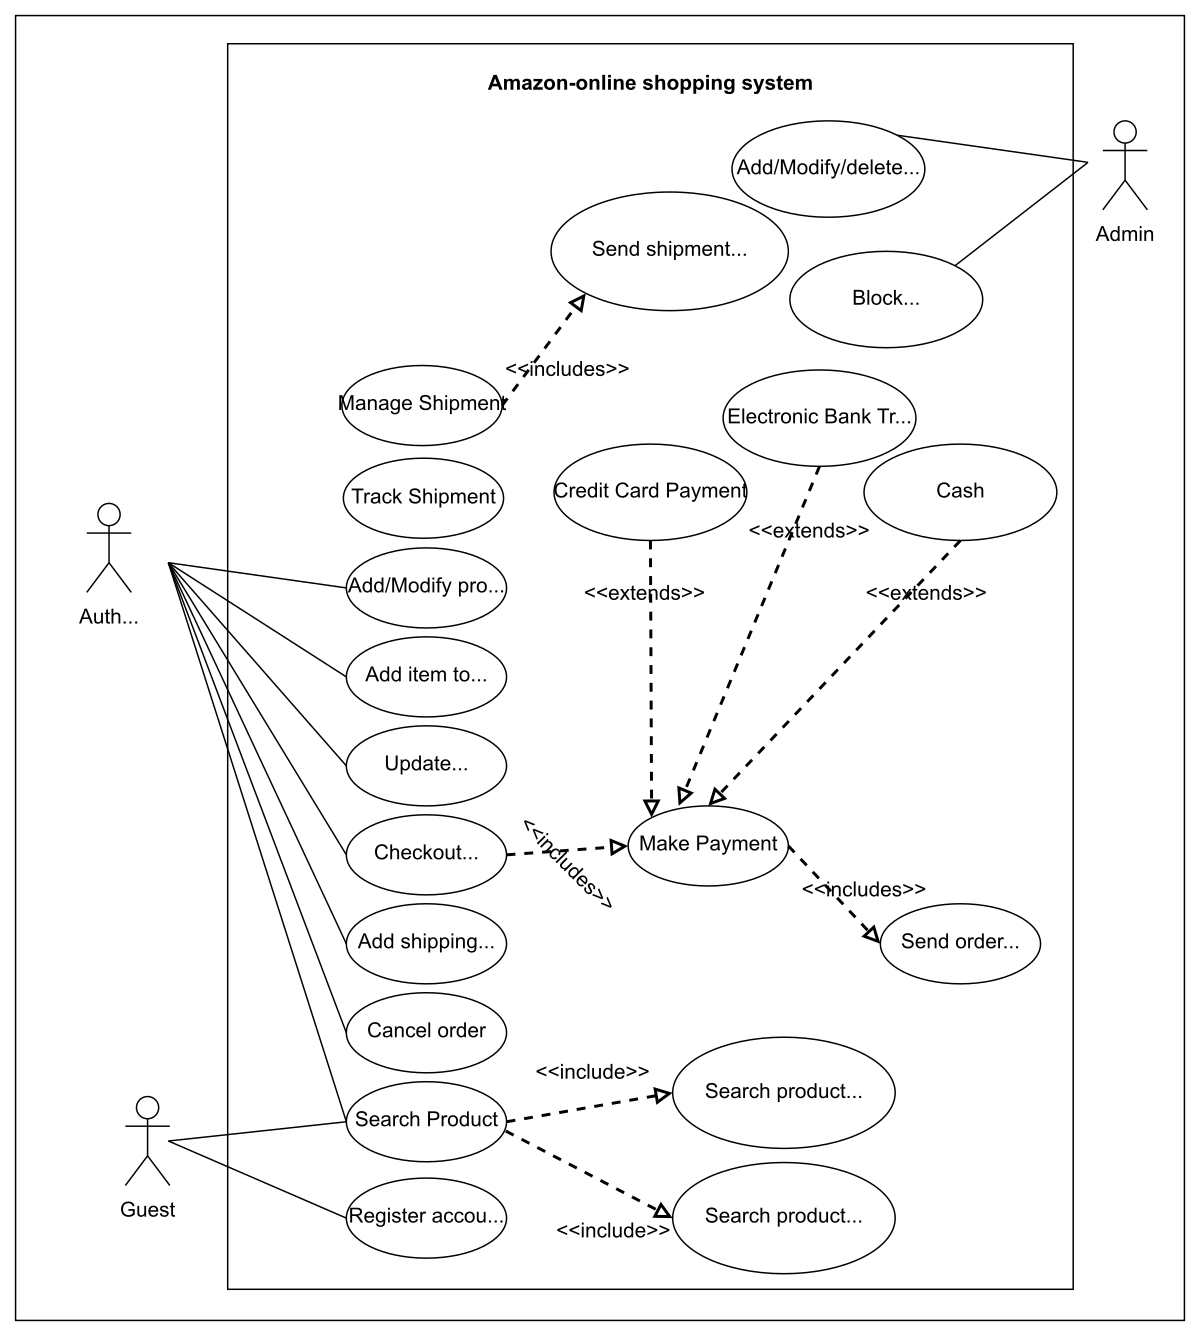
\includegraphics[width=0.5\textwidth]{Images/chapter_19/section_5402575537176576/5259421620764672.png}
 \caption{The use case diagram of the Amazon online shopping system}
\end{figure}

In the next lesson, we'll discuss the class diagram with a detailed explanation of all classes and their relationship with each other.

% End of section content